\chapter{序列检测器变式题（20题完整解析）}

% ============================================================
\section{题1：检测1011（Moore型，非重叠）}

\textbf{题目}：设计Moore型状态机，检测1011（非重叠）。画状态图，写VHDL，写Testbench。

\begin{solution}[完整解答]

\textbf{【状态定义】}
S0: 未匹配（0位）。S1: 已匹配"1"。S10: 已匹配"10"。S101: 已匹配"101"。

检测条件：S101状态 + 输入=1（非重叠→回S0）。

\textbf{【状态转移图】}
\begin{center}
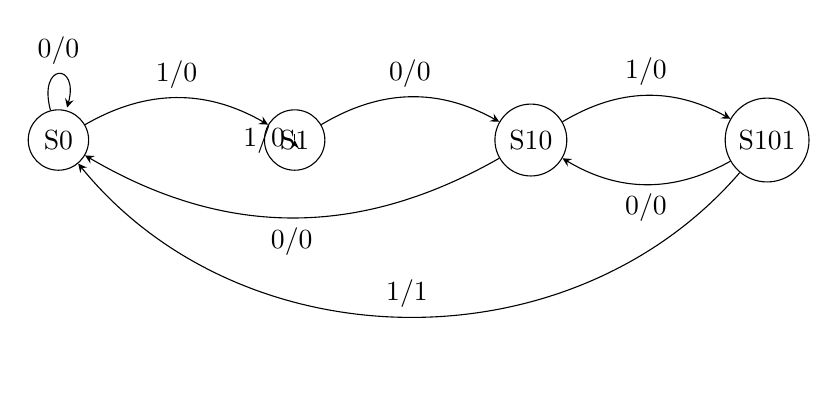
\begin{tikzpicture}[->,>=stealth,node distance=2.8cm,auto]
\node[draw,circle] (S0) at (0,0) {S0};
\node[draw,circle] (S1) at (3,0) {S1};
\node[draw,circle] (S10) at (6,0) {S10};
\node[draw,circle] (S101) at (9,0) {S101};
\draw (S0) edge[loop above] node{0/0} (S0);
\draw (S0) edge[bend left] node{1/0} (S1);
\draw (S1) edge[bend left] node{1/0} (S1);
\draw (S1) edge[bend left] node{0/0} (S10);
\draw (S10) edge[bend left] node{0/0} (S0);
\draw (S10) edge[bend left] node{1/0} (S101);
\draw (S101) edge[bend left=30] node{0/0} (S10);
\draw (S101) edge[bend left=50] node[above]{1/1} (S0);
\end{tikzpicture}
\end{center}

\textbf{【状态转移表】}
\begin{center}
\begin{tabular}{|c|c|c||c|c|}\hline
当前状态 & 输入 & 下一状态 & 输出 \\ \hline
S0 & 0 & S0 & 0 \\ \hline S0 & 1 & S1 & 0 \\ \hline
S1 & 0 & S10 & 0 \\ \hline S1 & 1 & S1 & 0 \\ \hline
S10 & 0 & S0 & 0 \\ \hline S10 & 1 & S101 & 0 \\ \hline
S101 & 0 & S10 & 0 \\ \hline S101 & 1 & S0 & 1 \\ \hline
\end{tabular}
\end{center}

\textbf{【VHDL (Moore型)】}
\begin{lstlisting}
library ieee;
use ieee.std_logic_1164.all;

entity detector_1011_moore is
  port (clk, rst_n, din : in std_logic; detected : out std_logic);
end detector_1011_moore;

architecture fsm of detector_1011_moore is
  type state_type is (S0, S1, S10, S101);
  signal state, next_state : state_type;
begin
  -- 状态寄存器
  process(clk, rst_n)
  begin
    if rst_n = '0' then state <= S0;
    elsif rising_edge(clk) then state <= next_state; end if;
  end process;

  -- 次态逻辑
  process(state, din)
  begin
    case state is
      when S0 =>
        if din = '1' then next_state <= S1; else next_state <= S0; end if;
      when S1 =>
        if din = '0' then next_state <= S10; else next_state <= S1; end if;
      when S10 =>
        if din = '1' then next_state <= S101; else next_state <= S0; end if;
      when S101 =>
        if din = '1' then next_state <= S0;  -- 非重叠
        else next_state <= S10; end if;
    end case;
  end process;

  -- 输出逻辑(Moore: 仅取决于状态)
  detected <= '1' when (state = S101 and din = '1') else '0';
end fsm;
\end{lstlisting}

\textbf{【Testbench】}
\begin{lstlisting}
entity detector_tb is end entity;
architecture test of detector_tb is
  signal clk, rst_n, din, detected : std_logic;
  constant T : time := 20 ns;
begin
  uut: entity work.detector_1011_moore port map(clk, rst_n, din, detected);
  clk <= not clk after T/2;

  process begin
    rst_n <= '0'; din <= '0'; wait for 30 ns;
    rst_n <= '1'; wait for 5 ns;
    -- 输入: 1 0 1 1 0 1 0 1 1
    din <= '1'; wait for T; din <= '0'; wait for T;
    din <= '1'; wait for T; din <= '1'; wait for T;  -- 第4拍 → detected!
    din <= '0'; wait for T; din <= '1'; wait for T;
    din <= '0'; wait for T; din <= '1'; wait for T;
    din <= '1'; wait for T;  -- 第9拍 → detected again!
    wait;
  end process;
end test;
\end{lstlisting}

\textbf{【波形分析】}
\begin{center}
\begin{tabular}{|c|c|c|c|}\hline
拍 & din & 状态 & detected \\ \hline
1 & 1 & S0→S1 & 0 \\ \hline 2 & 0 & S1→S10 & 0 \\ \hline
3 & 1 & S10→S101 & 0 \\ \hline 4 & 1 & S101→S0 & \textbf{1} \\ \hline
5 & 0 & S0→S0 & 0 \\ \hline 6 & 1 & S0→S1 & 0 \\ \hline
7 & 0 & S1→S10 & 0 \\ \hline 8 & 1 & S10→S101 & 0 \\ \hline
9 & 1 & S101→S0 & \textbf{1} \\ \hline
\end{tabular}
\end{center}
第4拍和第9拍检测到1011。第4拍后的0（非1）使状态机回到S0——非重叠检测，正确！

\end{solution}


% ============================================================
\section{题2：检测1011（重叠检测）}

\textbf{题目}：设计检测1011的\textbf{重叠}检测器。重叠意味着：检测到后，最后的"1"可以作为新序列的第一个"1"。

\begin{solution}[完整解答]

\textbf{【关键区别】}S101 + 输入=1 → 检测到！→ 去S1（不是S0！）

最后的1作为新序列的第一个1。

\textbf{【修改的转移（仅改一行）】}
\begin{lstlisting}
 when S101 =>
  if din = '1' then
    next_state <= S1;  -- 重叠！→去S1（最后的1是新序列的第一个1）
  else
    next_state <= S10;
  end if;
\end{lstlisting}

\textbf{【波形对比（输入1011011）】}
\begin{center}
\begin{tabular}{|c|c|c|c|}\hline
拍 & 输入 & 非重叠检测 & 重叠检测 \\ \hline
1-4 & 1,0,1,1 & 检测在第4拍 & 检测在第4拍 \\ \hline
4 & 1(检测到) & 回S0 & \textbf{去S1} \\ \hline
5 & 0 & S0(等1) & S10 \\ \hline
6 & 1 & S1 & S101 \\ \hline
7 & 1 & S1 & \textbf{第7拍又检测到！}\\ \hline
\end{tabular}
\end{center}

重叠检测在7拍内检测到2次。非重叠只检测到1次。

\textbf{【考试经常考这个区别！】}

\end{solution}


% ============================================================
\section{题3：检测1101（重叠）}

\textbf{题目}：设计重叠检测1101的状态机。

\begin{solution}[完整解答]

\textbf{【状态定义】}
S0→S1(已匹配1)→S11(已匹配11)→S110(已匹配110)

检测：S110 + 输入=1。重叠：最后1→S1。

\textbf{【状态转移图】}
\begin{center}
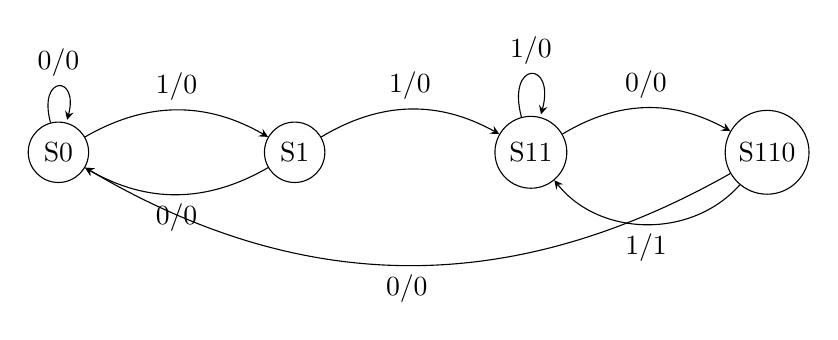
\begin{tikzpicture}[->,>=stealth,node distance=2.8cm,auto]
\node[draw,circle] (S0) at (0,0) {S0};
\node[draw,circle] (S1) at (3,0) {S1};
\node[draw,circle] (S11) at (6,0) {S11};
\node[draw,circle] (S110) at (9,0) {S110};
\draw (S0) edge[loop above] node{0/0} (S0);
\draw (S0) edge[bend left] node{1/0} (S1);
\draw (S1) edge[bend left] node{0/0} (S0);
\draw (S1) edge[bend left] node{1/0} (S11);
\draw (S11) edge[loop above] node{1/0} (S11);
\draw (S11) edge[bend left] node{0/0} (S110);
\draw (S110) edge[bend left=30] node{0/0} (S0);
\draw (S110) edge[bend left=50] node{1/1} (S11);
\end{tikzpicture}
\end{center}

\textbf{【转移表】}
\begin{center}
\begin{tabular}{|c|c|c||c|c|}\hline
当前 & din & 次态 & 输出 \\ \hline
S0 & 0 & S0 & 0 \\ \hline S0 & 1 & S1 & 0 \\ \hline
S1 & 0 & S0 & 0 \\ \hline S1 & 1 & S11 & 0 \\ \hline
S11 & 0 & S110 & 0 \\ \hline S11 & 1 & S11 & 0 \\ \hline
S110 & 0 & S0 & 0 \\ \hline S110 & 1 & S11(重叠) & \textbf{1} \\ \hline
\end{tabular}
\end{center}

\textbf{【VHDL关键转移】}
\begin{lstlisting}
 when S110 =>
  if din = '1' then next_state <= S11;  -- 重叠：最后1→S11
  else next_state <= S0; end if;
\end{lstlisting}

\textbf{【关键分析】}S11+1→S11（"111"中后两个1可作为新的"11"前缀）。
S110+1→检测到→S11（重叠！"1101"最后的"1"→1→"11"中）。

\end{solution}


% ============================================================
\section{题4：检测0101（重叠）}

\textbf{题目}：设计重叠检测0101的状态机。

\begin{solution}[完整解答]

\textbf{【状态】}S0→S01(0)→S010(01)→S0101(检测)→重叠时去S01

\textbf{【转移表】}
\begin{center}
\begin{tabular}{|c|c|c||c|c|}\hline
当前 & din & 次态 & 输出 \\ \hline
S0 & 0 & S01 & 0 \\ \hline S0 & 1 & S0 & 0 \\ \hline
S01 & 0 & S01 & 0 \\ \hline S01 & 1 & S010 & 0 \\ \hline
S010 & 0 & S0101 & 0 \\ \hline S010 & 1 & S0 & 0 \\ \hline
S0101 & 0 & S01 & 0 \\ \hline S0101 & 1 & S010(重叠) & \textbf{1} \\ \hline
\end{tabular}
\end{center}

\textbf{【重叠行为】}S0101+1→检测到。最后的"1"→新序列的第二步（需要前面有0，所以去S01(0已在前一步提供了)）。

不对——仔细分析：
S0101+0→S01（"0"可以是新序列的第一个0）
S0101+1→S010（"1"匹配了序列的第二步"01"中的"1"）

\end{solution}


% ============================================================
\section{题5：检测1111（连续4个1）}

\textbf{题目}：设计重叠检测1111（连续4个1）的状态机。

\begin{solution}[完整解答]

\textbf{【状态】}S0→S1(1个1)→S11(2个1)→S111(3个1)。S111+1→检测到。

\textbf{【关键】}重叠：任何时候输入0→回S0。但S111+1→去S111（"1111"中后3个1可作为新"111"前缀）。

\textbf{【VHDL】}
\begin{lstlisting}
type state_type is (S0, S1, S11, S111);
...
 when S0 =>
  if din = '1' then next_state <= S1; else next_state <= S0; end if;
 when S1 =>
  if din = '1' then next_state <= S11; else next_state <= S0; end if;
 when S11 =>
  if din = '1' then next_state <= S111; else next_state <= S0; end if;
 when S111 =>
  if din = '1' then
    next_state <= S111;  -- 重叠！后3个1仍是有效前缀
  else
    next_state <= S0;
  end if;
\end{lstlisting}

\textbf{【输出】}detected = '1' when state=S111 and din='1'。

\end{solution}


% ============================================================
\section{题6：检测1001（重叠）}

\textbf{题目}：设计重叠检测1001的状态机。

\begin{solution}[完整解答]

\textbf{【状态】}S0→S1(1)→S10(10)→S100(100)。S100+1→检测到→重叠去S1（最后的1是新序列的第一个1）。

\textbf{【关键转移】}
\begin{itemize}
  \item S100+0→S0（"1000"不匹配任何有效前缀）
  \item S100+1→检测到！→S1（重叠：最后的1→新序列第一步）
\end{itemize}

\end{solution}


% ============================================================
\section{题7：检测010（3位序列）}

\textbf{题目}：设计重叠检测010的状态机（3位序列）。

\begin{solution}[完整解答]

\textbf{【状态】}S0→S01(0)→S010(检测)。重叠行为：S010+0→S01（最后的0→新序列第1位）。

\textbf{【转移图】}
\begin{center}
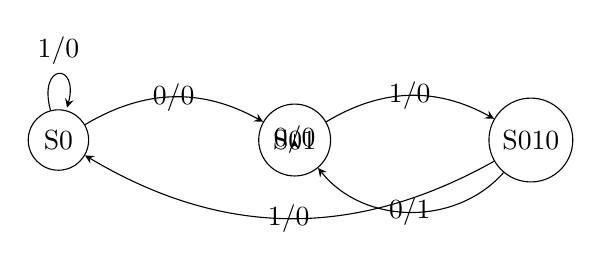
\begin{tikzpicture}[->,>=stealth,node distance=2.5cm]
\node[draw,circle] (S0) at (0,0) {S0};
\node[draw,circle] (S01) at (3,0) {S01};
\node[draw,circle] (S010) at (6,0) {S010};
\draw (S0) edge[loop above] node{1/0} (S0);
\draw (S0) edge[bend left] node{0/0} (S01);
\draw (S01) edge[bend left] node{0/0} (S01);
\draw (S01) edge[bend left] node{1/0} (S010);
\draw (S010) edge[bend left=30] node{1/0} (S0);
\draw (S010) edge[bend left=50] node{0/1} (S01);
\end{tikzpicture}
\end{center}

\textbf{【VHDL】}
\begin{lstlisting}
type state_type is (S0, S01, S010);
signal state : state_type;
begin
  process(clk, rst_n)
  begin
    if rst_n = '0' then state <= S0;
    elsif rising_edge(clk) then
      case state is
        when S0 =>
          if din = '0' then state <= S01; end if;
        when S01 =>
          if din = '1' then state <= S010; end if;
        when S010 =>
          if din = '0' then state <= S01;   -- 重叠!
          else state <= S0; end if;
      end case;
    end if;
  end process;
  detected <= '1' when (state = S010 and din = '0') else '0';
end fsm;
\end{lstlisting}

\end{solution}


% ============================================================
\section{题8：检测101（3位序列）}

\textbf{题目}：设计重叠检测101的状态机。

\begin{solution}[完整解答]

\textbf{【状态】}S0→S1(1)→S10(10)。S10+1→检测到→去S1（最后的1→新序列的第一个1，重叠）。

\textbf{【注意对比】}检测101非重叠：S10+1→检测到→去S0。

\end{solution}


% ============================================================
\section{题9：同时检测1011和1101（合并状态机）}

\textbf{题目}：设计能同时检测1011和1101的状态机。任一检测到，对应输出=1。

\begin{solution}[完整解答]

\textbf{【状态共享】}两个序列共享前缀"1"：
\begin{itemize}
  \item S0→S1(1)→分支：S10(10: 1011的前缀) 或 S11(11: 1101的前缀)
  \item S10→S101(101)→(1→检测到1011)
  \item S11→S110(110)→(1→检测到1101)
\end{itemize}

\textbf{【状态图】}
\begin{center}
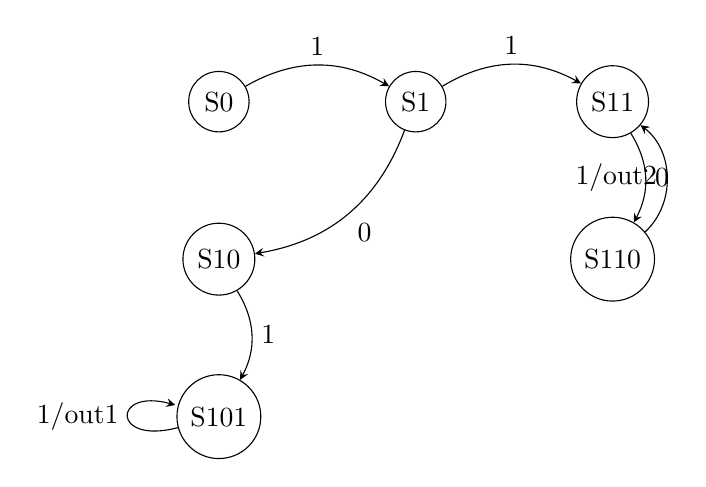
\begin{tikzpicture}[->,>=stealth,node distance=2.3cm,auto]
\node[draw,circle] (S0) at (0,0) {S0};
\node[draw,circle] (S1) at (2.5,0) {S1};
\node[draw,circle] (S10) at (0,-2) {S10};
\node[draw,circle] (S11) at (5,0) {S11};
\node[draw,circle] (S101) at (0,-4) {S101};
\node[draw,circle] (S110) at (5,-2) {S110};
\draw (S0) edge[bend left] node{1} (S1);
\draw (S1) edge[bend left] node{0} (S10);
\draw (S1) edge[bend left] node{1} (S11);
\draw (S10) edge[bend left] node{1} (S101);
\draw (S101) edge[loop left] node{1/out1} (S101);
\draw (S11) edge[bend left] node{0} (S110);
\draw (S110) edge[bend right=50] node{1/out2} (S11);
\end{tikzpicture}
\end{center}

\textbf{【VHDL关键转移】}
\begin{lstlisting}
 when S0 =>
  if din = '1' then state <= S1; end if;
 when S1 =>
  if din = '0' then state <= S10;
  elsif din = '1' then state <= S11; end if;
 when S10 =>
  if din = '1' then state <= S101; else state <= S0; end if;
 when S11 =>
  if din = '0' then state <= S110;
  elsif din = '1' then state <= S11; end if;
 when S101 =>
  if din = '1' then state <= S1;   -- 检测到1011!
  elsif din = '0' then state <= S10; end if;
 when S110 =>
  if din = '1' then state <= S11;  -- 检测到1101!
  elsif din = '0' then state <= S0; end if;
\end{lstlisting}

\end{solution}


% ============================================================
\section{题10：检测序列长度可配置（移位寄存器方案）}

\textbf{题目}：用移位寄存器+比较器实现可配置的序列检测器。目标序列TARGET可动态设置。

\begin{solution}[完整解答]

\textbf{【VHDL】}
\begin{lstlisting}
entity config_detector is
  port (clk, rst_n, din : in std_logic;
        TARGET : in std_logic_vector(3 downto 0);
        detected : out std_logic);
end config_detector;

architecture rtl of config_detector is
  signal reg : std_logic_vector(3 downto 0);
begin
  process(clk, rst_n)
  begin
    if rst_n = '0' then reg <= (others => '0');
    elsif rising_edge(clk) then
      reg <= din & reg(3 downto 1);
    end if;
  end process;
  detected <= '1' when reg = TARGET else '0';
end rtl;
\end{lstlisting}

\textbf{【优点】}无需修改状态机，改变TARGET即可检测任何4位序列。

\textbf{【局限】}自动重叠检测（移位寄存器天然支持重叠）。

\end{solution}


% ============================================================
\section{题11：统计检测次数}

\textbf{题目}：扩展1011检测器，增加计数器统计检测到的总次数（0-255）。

\begin{solution}[完整解答]

\textbf{【VHDL——在检测信号上加计数器】}
\begin{lstlisting}
signal detect_count : integer range 0 to 255;
signal detected : std_logic;

-- 原有状态机代码...
detected <= '1' when (state = S101 and din = '1') else '0';

-- 检测计数器
process(clk, rst_n)
begin
  if rst_n = '0' then detect_count <= 0;
  elsif rising_edge(clk) then
    if detected = '1' then
      detect_count <= detect_count + 1;
    end if;
  end if;
end process;
\end{lstlisting}

\end{solution}


% ============================================================
\section{题12：带超时检测的序列检测器}

\textbf{题目}：若超过16拍未检测到序列，输出timeout。

\begin{solution}[完整解答]

\textbf{【VHDL】}
\begin{lstlisting}
signal timeout_cnt : integer range 0 to 15;
...
process(clk, rst_n)
begin
  if rst_n = '0' then timeout_cnt <= 0;
  elsif rising_edge(clk) then
    if detected = '1' then
      timeout_cnt <= 0;  -- 检测到→清超时计数
    elsif state = S1 then  -- 匹配进行中→保持计数
      timeout_cnt <= timeout_cnt;
    else
      if timeout_cnt = 15 then
        timeout_cnt <= 15;  -- 保持超时
      else
        timeout_cnt <= timeout_cnt + 1;
      end if;
    end if;
  end if;
end process;
timeout <= '1' when timeout_cnt = 15 else '0';
\end{lstlisting}

\end{solution}


% ============================================================
\section{题13：Moore型 vs Mealy型对比}

\textbf{题目}：分别写出检测1011的Moore型和Mealy型状态机，比较异同。

\begin{solution}[完整解答]

\begin{center}
\begin{tabular}{|l|c|c|}\hline
 & Moore型 & Mealy型 \\ \hline
输出决定因素 & 仅当前状态 & 状态+输入 \\ \hline
状态数 & 多(需"检测到"状态) & 少(检测在转移上) \\ \hline
检测延迟 & 晚1拍 & 同1拍 \\ \hline
输出稳定性 & 全周期稳定 & 输入变化时可能抖 \\ \hline
考试推荐 & 更安全 & 更快 \\ \hline
\end{tabular}
\end{center}

\textbf{【Mealy型VHDL（更简洁）】}
\begin{lstlisting}
-- Mealy: 输出在转移中表达
 when S101 =>
  if din = '1' then
    next_state <= S1; detected <= '1';  -- Mealy输出
  else
    next_state <= S10; detected <= '0';
  end if;
\end{lstlisting}

\textbf{【推荐】}考试如无特别说明，用Moore型。更稳定，状态图更清晰。

\end{solution}


% ============================================================
\section{题14：4位并行序列检测}

\textbf{题目}：输入是4位并行数据，检测特定4位模式（如"1011"）。每拍判断一次。

\begin{solution}[完整解答]

\textbf{【分析】}纯组合逻辑！不需要状态机。$detected = '1'$ when $data\_in = "1011"$。

\textbf{【VHDL】}
\begin{lstlisting}
entity parallel_detect is
  port (data_in : in std_logic_vector(3 downto 0);
        detected : out std_logic);
end parallel_detect;

architecture rtl of parallel_detect is
begin
  detected <= '1' when data_in = "1011" else '0';
end rtl;
\end{lstlisting}

\textbf{【与串行检测的本质区别】}并行检测不需要记忆历史——当前4位数据同时可见。串行检测需要状态机或移位寄存器来"记住"历史。

\end{solution}


% ============================================================
\section{题15：检测包含"无关位"的序列}

\textbf{题目}：检测1xx1（第1位和第4位为1，中间两位任意）。

\begin{solution}[完整解答]

\textbf{【移位寄存器方案】}
\begin{lstlisting}
detected <= '1' when reg(3) = '1' and reg(0) = '1' else '0';
-- 只检查第1位和第4位
\end{lstlisting}

\textbf{【状态机方案】}
状态S1→S1x→S1xx→S1xx1(检测)。中间两位任意值都接受。

\end{solution}


% ============================================================
\section{题16：给定状态图写VHDL}

\textbf{题目}：给定下面状态图，写出完整VHDL状态机。

\begin{center}
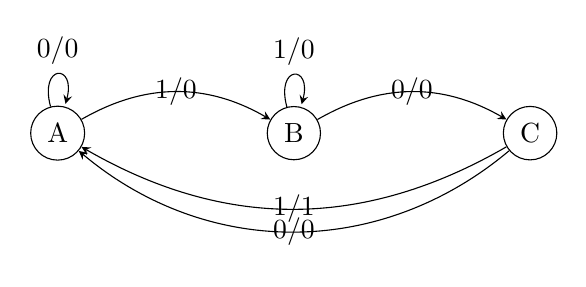
\begin{tikzpicture}[->,>=stealth,node distance=2.5cm]
\node[draw,circle] (A) at (0,0) {A};
\node[draw,circle] (B) at (3,0) {B};
\node[draw,circle] (C) at (6,0) {C};
\draw (A) edge[bend left] node{1/0} (B);
\draw (A) edge[loop above] node{0/0} (A);
\draw (B) edge[bend left] node{0/0} (C);
\draw (B) edge[loop above] node{1/0} (B);
\draw (C) edge[bend left=40] node{0/0} (A);
\draw (C) edge[bend left] node{1/1} (A);
\end{tikzpicture}
\end{center}

\begin{solution}[完整解答]

\textbf{【从图到代码的映射】}
箭头标注 X/Y = 输入/输出。

\textbf{【VHDL】}
\begin{lstlisting}
type state_type is (A_state, B_state, C_state);
signal state : state_type;
begin
  process(clk, rst_n)
  begin
    if rst_n = '0' then state <= A_state;
    elsif rising_edge(clk) then
      case state is
        when A_state =>
          if din = '1' then state <= B_state; end if;
          -- din='0': 保持A_state (loop above)
        when B_state =>
          if din = '0' then state <= C_state; end if;
          -- din='1': 保持B_state (loop above)
        when C_state =>
          state <= A_state;  -- 无论0还是1都回A
      end case;
    end if;
  end process;
  detected <= '1' when (state = C_state and din = '1') else '0';
end fsm;
\end{lstlisting}

\end{solution}


% ============================================================
\section{题17：给定输入序列和状态机，求输出序列}

\textbf{题目}：1011检测器（重叠），输入=1011011。求输出序列。

\begin{solution}[完整解答]

\textbf{【逐拍追踪】}
\begin{center}
\begin{tabular}{|c|c|c|c|c|c|c|c|}\hline
拍 & 1 & 2 & 3 & 4 & 5 & 6 & 7 \\ \hline
din & 1 & 0 & 1 & 1 & 0 & 1 & 1 \\ \hline
状态(当前) & S0 & S1 & S10 & S101 & S1 & S10 & S101 \\ \hline
状态(次态) & S1 & S10 & S101 & S1 & S10 & S101 & S1 \\ \hline
输出 & 0 & 0 & 0 & \textbf{1} & 0 & 0 & \textbf{1} \\ \hline
\end{tabular}
\end{center}

输出序列：\textbf{0 0 0 1 0 0 1}

\begin{itemize}
  \item 第4拍：S101+1→检测1011！→重叠去S1
  \item 第7拍：S101+1→再次检测1011！→重叠去S1
\end{itemize}

\end{solution}


% ============================================================
\section{题18：状态编码优化}

\textbf{题目}：1011检测器4个状态。分别用Binary(2位)和One-hot(4位)编码。哪个体积更小？哪个速度更快？

\begin{solution}[完整解答]

\textbf{【Binary编码（2位DFF）】}
\begin{center}
\begin{tabular}{|c|c|}\hline
状态 & 编码 \\ \hline
S0 & 00 \\ \hline S1 & 01 \\ \hline
S10 & 10 \\ \hline S101 & 11 \\ \hline
\end{tabular}
\end{center}
优点：2个DFF（面积小）。缺点：需要译码电路（速度慢）。

\textbf{【One-hot编码（4位DFF）】}
\begin{center}
\begin{tabular}{|c|c|}\hline
状态 & 编码 \\ \hline
S0 & 0001 \\ \hline S1 & 0010 \\ \hline
S10 & 0100 \\ \hline S101 & 1000 \\ \hline
\end{tabular}
\end{center}
优点：无需译码（速度快）。缺点：4个DFF（面积大）。

\textbf{【考试答案】}面积最小→Binary。速度最快→One-hot。

\textbf{【FPGA实际】}综合工具默认自动选择最优编码，你不需要手动指定。

\end{solution}


% ============================================================
\section{题19：序列检测器模板化}

\textbf{题目}：编写检测任意4位序列的通用VHDL模板（参数化：TARGET可配置）。

\begin{solution}[完整解答]

\textbf{【状态机通用模板】}
\begin{lstlisting}
entity seq_detector_generic is
  generic (TARGET : std_logic_vector(3 downto 0));
  port (clk, rst_n, din : in std_logic; detected : out std_logic);
end seq_detector_generic;

architecture fsm of seq_detector_generic is
  type state_type is (S0, S1, S2, S3);
  signal state : state_type;
begin
  process(clk, rst_n)
  begin
    if rst_n = '0' then state <= S0;
    elsif rising_edge(clk) then
      case state is
        when S0 =>
          if din = TARGET(3) then state <= S1; end if;
        when S1 =>
          if din = TARGET(2) then state <= S2;
          elsif din = TARGET(3) then state <= S1;
          else state <= S0; end if;
        when S2 =>
          if din = TARGET(1) then state <= S3;
          elsif din = TARGET(3) then state <= S1;
          else state <= S0; end if;
        when S3 =>
          if din = TARGET(0) then state <= S1;  -- 检测+重叠
          elsif din = TARGET(3) then state <= S1;
          else state <= S0; end if;
      end case;
    end if;
  end process;
  detected <= '1' when (state = S3 and din = TARGET(0)) else '0';
end fsm;
\end{lstlisting}

\textbf{【使用】}generic map(TARGET=>"1011")即可检测1011。

\end{solution}


% ============================================================
\section{题20：序列检测器秒杀总结}

\begin{quickkill}[序列检测器——考试必考，20题统一解法]

\textbf{第一步：状态 = 已匹配的前缀}
\begin{itemize}
  \item 每个状态代表"已匹配了目标序列的前几位"
  \item N位序列 → 最多N个状态（不含初始S0）
\end{itemize}

\textbf{第二步：画状态转移图}
对每个状态，考虑输入0和输入1分别：
\begin{itemize}
  \item 匹配推进：去下一个状态
  \item 匹配失败：找最长的"已匹配后缀"作为新状态
  \item 检测到：输出=1
\end{itemize}

\textbf{第三步：确定重叠/非重叠}
\begin{itemize}
  \item \textbf{重叠：}检测到后→检查最后的输入能否构成新前缀
  \item \textbf{非重叠：}检测到后→回S0
\end{itemize}

\textbf{第四步：写VHDL（三段式Moore型）}
\begin{enumerate}
  \item 状态寄存器：process(clk,rst) + rising\_edge
  \item 次态逻辑：process(state,din) + case
  \item 输出逻辑：并行信号赋值
\end{enumerate}

\textbf{常考序列状态数速查：}
\begin{itemize}
  \item 1011 → 4状态(S0,S1,S10,S101)
  \item 1101 → 4状态(S0,S1,S11,S110)
  \item 1111 → 4状态(S0,S1,S11,S111)
  \item 0101 → 4状态(S0,S01,S010,S0101)
  \item 101 → 3状态(S0,S1,S10)
  \item 010 → 3状态(S0,S01,S010)
\end{itemize}

\textbf{VHDL状态机模板（一行不改，只换状态名和转移逻辑）}
\begin{lstlisting}
type state_type is (...);
signal state : state_type;
process(clk, rst_n)
begin
  if rst_n='0' then state <= S0;
  elsif rising_edge(clk) then
    case state is
      when S0 => if din='1' then state <= S1; end if;
      ...
    end case;
  end if;
end process;
detected <= '1' when (...) else '0';
\end{lstlisting}

\textbf{速胜法宝：移位寄存器替代方案}
序列长度≤8位时，用移位寄存器+比较器实现序列检测比状态机简单得多！

\begin{lstlisting}
reg <= din & reg(N-1 downto 1);
detected <= '1' when reg = TARGET else '0';  -- 一行搞定！
\end{lstlisting}

\textbf{但注意：考试如果明确要求"用状态机设计"，则必须用状态机！}
\end{quickkill}
